This chapter gives a brief introduction to the content of the project through presenting the motivation behind it, and statement of the goals.
    \section{Motivation}
In a world hooked on technologies, a connection to the outside world is crucial, even when a person is in the car. This is the reason behind every car manufacturer trying to come up with some technological ecosystem that won’t just connect the car, but also the user to the world around him.
BMW technology package called ConnectedDrive has currently over 8 million cars that connect daily to almost 300 micro services that guarantee not only entertainment but most importantly the security of the users. This services range from Map Updates to Real Time Traffic Information to Concierge Services. Due to such a diversified range with high utility for the user, the cars become moving data centers.
Aggregating these connections by time, one type of data that results is represented in the form of requests to connect to BMW servers (to get access the the mentioned services)  per second (requests/sec)\footnote{https://www.bmw-connecteddrive.de/app/index.html\#/portal/store}. 
Having such huge amounts of data generated continuously, a daily pattern can be observed that corresponds to the intuitive rush-hour peaks.
\begin{figure}[h]
    \centering
    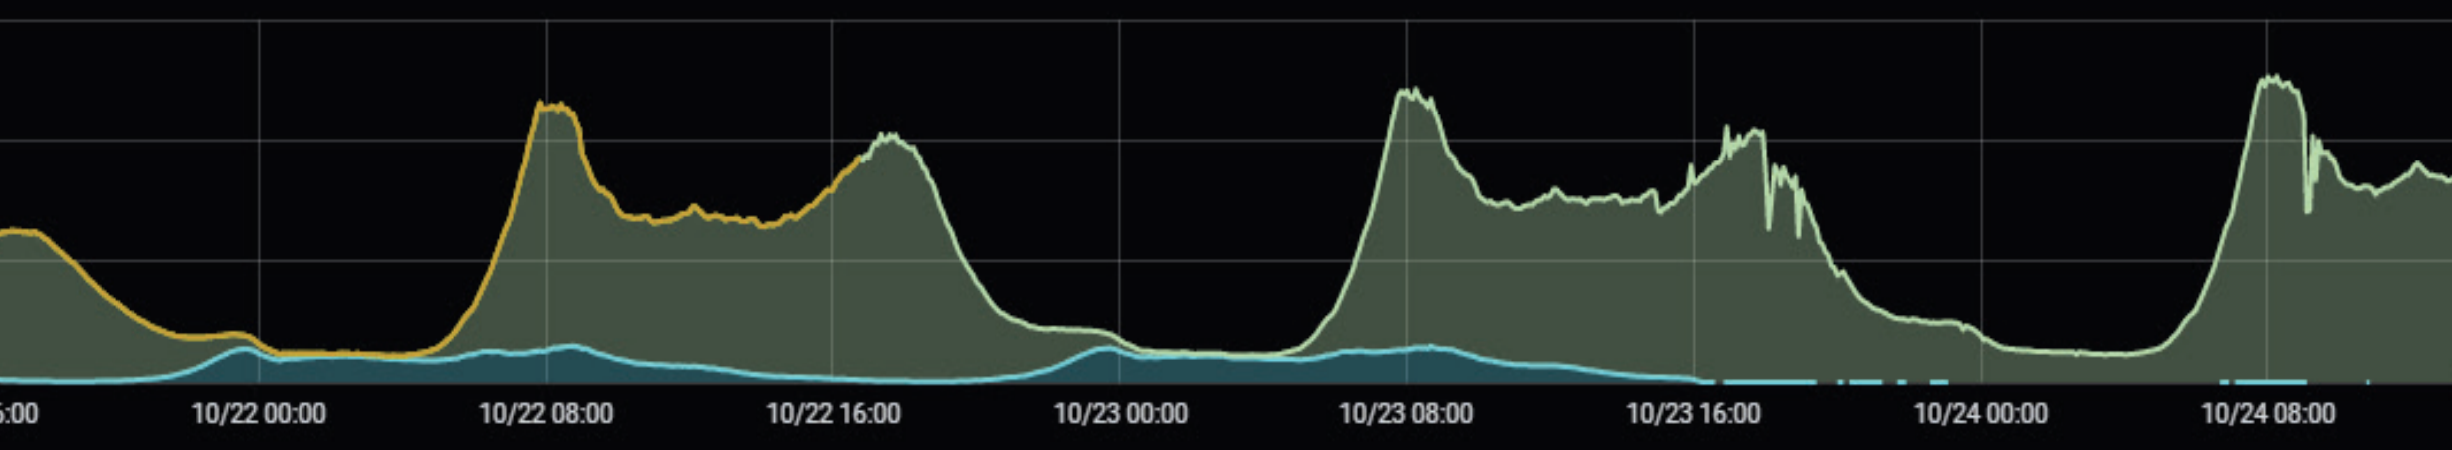
\includegraphics[width=1\textwidth]{images/data-graph.png}
    \caption{Visualisation of BMW data in form of requests per second }
\end{figure}

    \section{Goals}
The primary goal of this project is to develop a framework, based on AWS service, that would be able to detect in a real-time environment a deviation from the pattern mentioned above, label it as an anomaly, and escalate a notification to a tool, e.g. a Slack channel, in the form of an alert accompanied by a small visual representation of the problem.\\
As a secondary challenge, the project attempts to incorporate a prediction feature, that would deliver information which would allow for predictive scaling of the infrastructure based on a generated short-term prognosis. The purpose of this feature has a deeply financial reasoning behind, allowing the team to adapt the infrastructure besed on the predicted needs, thus reducing the expenses with the AWS services. \\
The final goal of the project was to come up with an additional set of recommendations and potential improvements to the delivered product.  This list of future features that can be investigated by the BMW team in order to assess the prospective value of adding them to their existing framework.